% potřeba:
% \usetikzlibrary{arrows.meta,positioning,shapes.geometric}

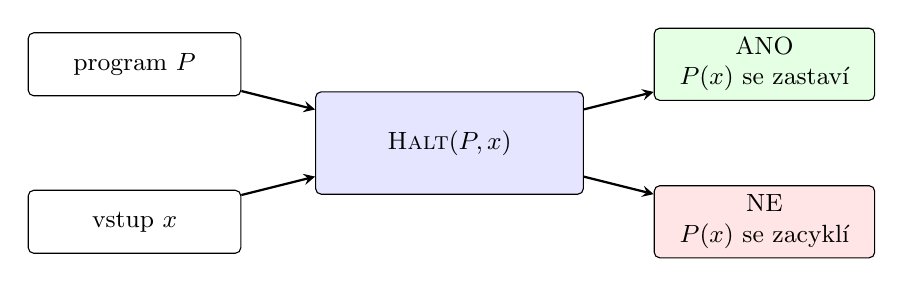
\begin{tikzpicture}[
    >=stealth,
    every node/.style={font=\small},
    box/.style={
        draw,
        rounded corners=2pt,
        align=center,
        minimum width=2.7cm,
        minimum height=8mm
    },
    bigbox/.style={
        draw,
        rounded corners=2pt,
        align=center,
        minimum width=3.4cm,
        minimum height=13mm
    },
    outbox/.style={
        draw,
        rounded corners=2pt,
        align=center,
        minimum width=2.8cm,
        minimum height=8mm
    }
]

% vstupy
\node[box] (prog) at (0,1.0) {program $P$};
\node[box] (inp)  at (0,-1.0) {vstup $x$};

% rozhodovací procedura
\node[bigbox, fill=blue!10] (halt) at (4,0) {$\textsc{Halt}(P,x)$};

% výstupy
\node[outbox, fill=green!10] (yes) at (8,1.0) {\markdarkgreen{ANO}\\$P(x)$ se zastaví};
\node[outbox, fill=red!10]   (no)  at (8,-1.0) {\markdarkred{NE}\\$P(x)$ se zacyklí};

% šipky
\draw[->, thick] (prog) -- (halt);
\draw[->, thick] (inp) -- (halt);
\draw[->, thick] (halt) -- (yes);
\draw[->, thick] (halt) -- (no);

\end{tikzpicture}